\section{Appendix}
\subsection{Energy-based approach algorithm}
\label{ch7:sect:App_energyBasedAlg}

The pseudo code of the energy-based physics injection flow matching algorithm involving full and intermediate trajectory injection strategies is described in Algorithm~\ref{ch7:alg:energyAlg}.

\begin{algorithm}[H]
\caption{Energy-based Guided Flow Matching}
\begin{algorithmic}[1]
\Require Pretrained velocity field $u_t^\theta$, energy $\mathcal{E}(\cdot)$, coefficient $\lambda$, total steps $T$, cutoff time $t_c\in[0,1]$
\State Set $\Delta t = 1/T$
\State Initialize $\mathbf{x}_0 \sim \mathcal{N}(0,I)$
\For{$i = 0$ to $T-1$}
    \State $t_i = i\,\Delta t$
    \If{$t_i < t_c$}  
        \State $\dot{\mathbf{x}} \leftarrow u_{t_i}^\theta(\mathbf{x}_i, t_i)$
    \Else
        \State $\dot{\mathbf{x}} \leftarrow u_{t_i}^\theta(\mathbf{x}_i, t_i)\;-\;\lambda\,\nabla_{\mathbf{x}_i}\mathcal{E}(\mathbf{x}_i)$
    \EndIf
    \State $\mathbf{x}_{i+1} \leftarrow \mathbf{x}_i + \Delta t\,\dot{\mathbf{x}}$
\EndFor
\State \Return $\mathbf{x}_1$
\end{algorithmic}
\label{ch7:alg:energyAlg}
\end{algorithm}


\subsection{Airfoil case}
\subsubsection{Model performance}
\label{ch7:subsect:modelPerformance}
We present the model performance comparative study results in Table~\ref{ch7:tab:modelPerformanceResults}. We primarily compare the final reduced values of the physical loss $\mathcal{L}_{\mathrm{phys}}$, the achieved $C_{L}$ accuracy, and the computation time. To ensure a fair comparison involving the surrogate model, all experiments are conducted on CPUs. In summary, \textit{Dflow-SUR} demonstrates a four orders-of-magnitude improvement in physical loss and achieves an approximate $74.47\%$ reduction in runtime compared to the energy-based baseline (with $t_c = 0.6$ and $T = 1000$), highlighting its exceptional capability to learn and enforce physical constraints.

\subsubsection{Gradient alignment score}
We further present the gradient alignment score of the energy-based approach when $t_c = 0.20, 0.60, 0.80$ (introduced in Section~\ref{ch7:subsect:physicalloss}) in Figure~\ref{ch7:fig:alignmentScore_app}. It can be observed that the gradient collision phenomenon persists during the primary inference phase. This indicates that the physical loss and flow matching loss consistently compete in their influence on design $\textbf{x}$, a behavior attributable to the issues arising from the injection of two guidance couplings.

\label{ch7:sect:gradientAlignmentScore}
\begin{figure}[htbp]
    \centering
    \subfloat[Physics injection when $t_c=0.2$]{%
        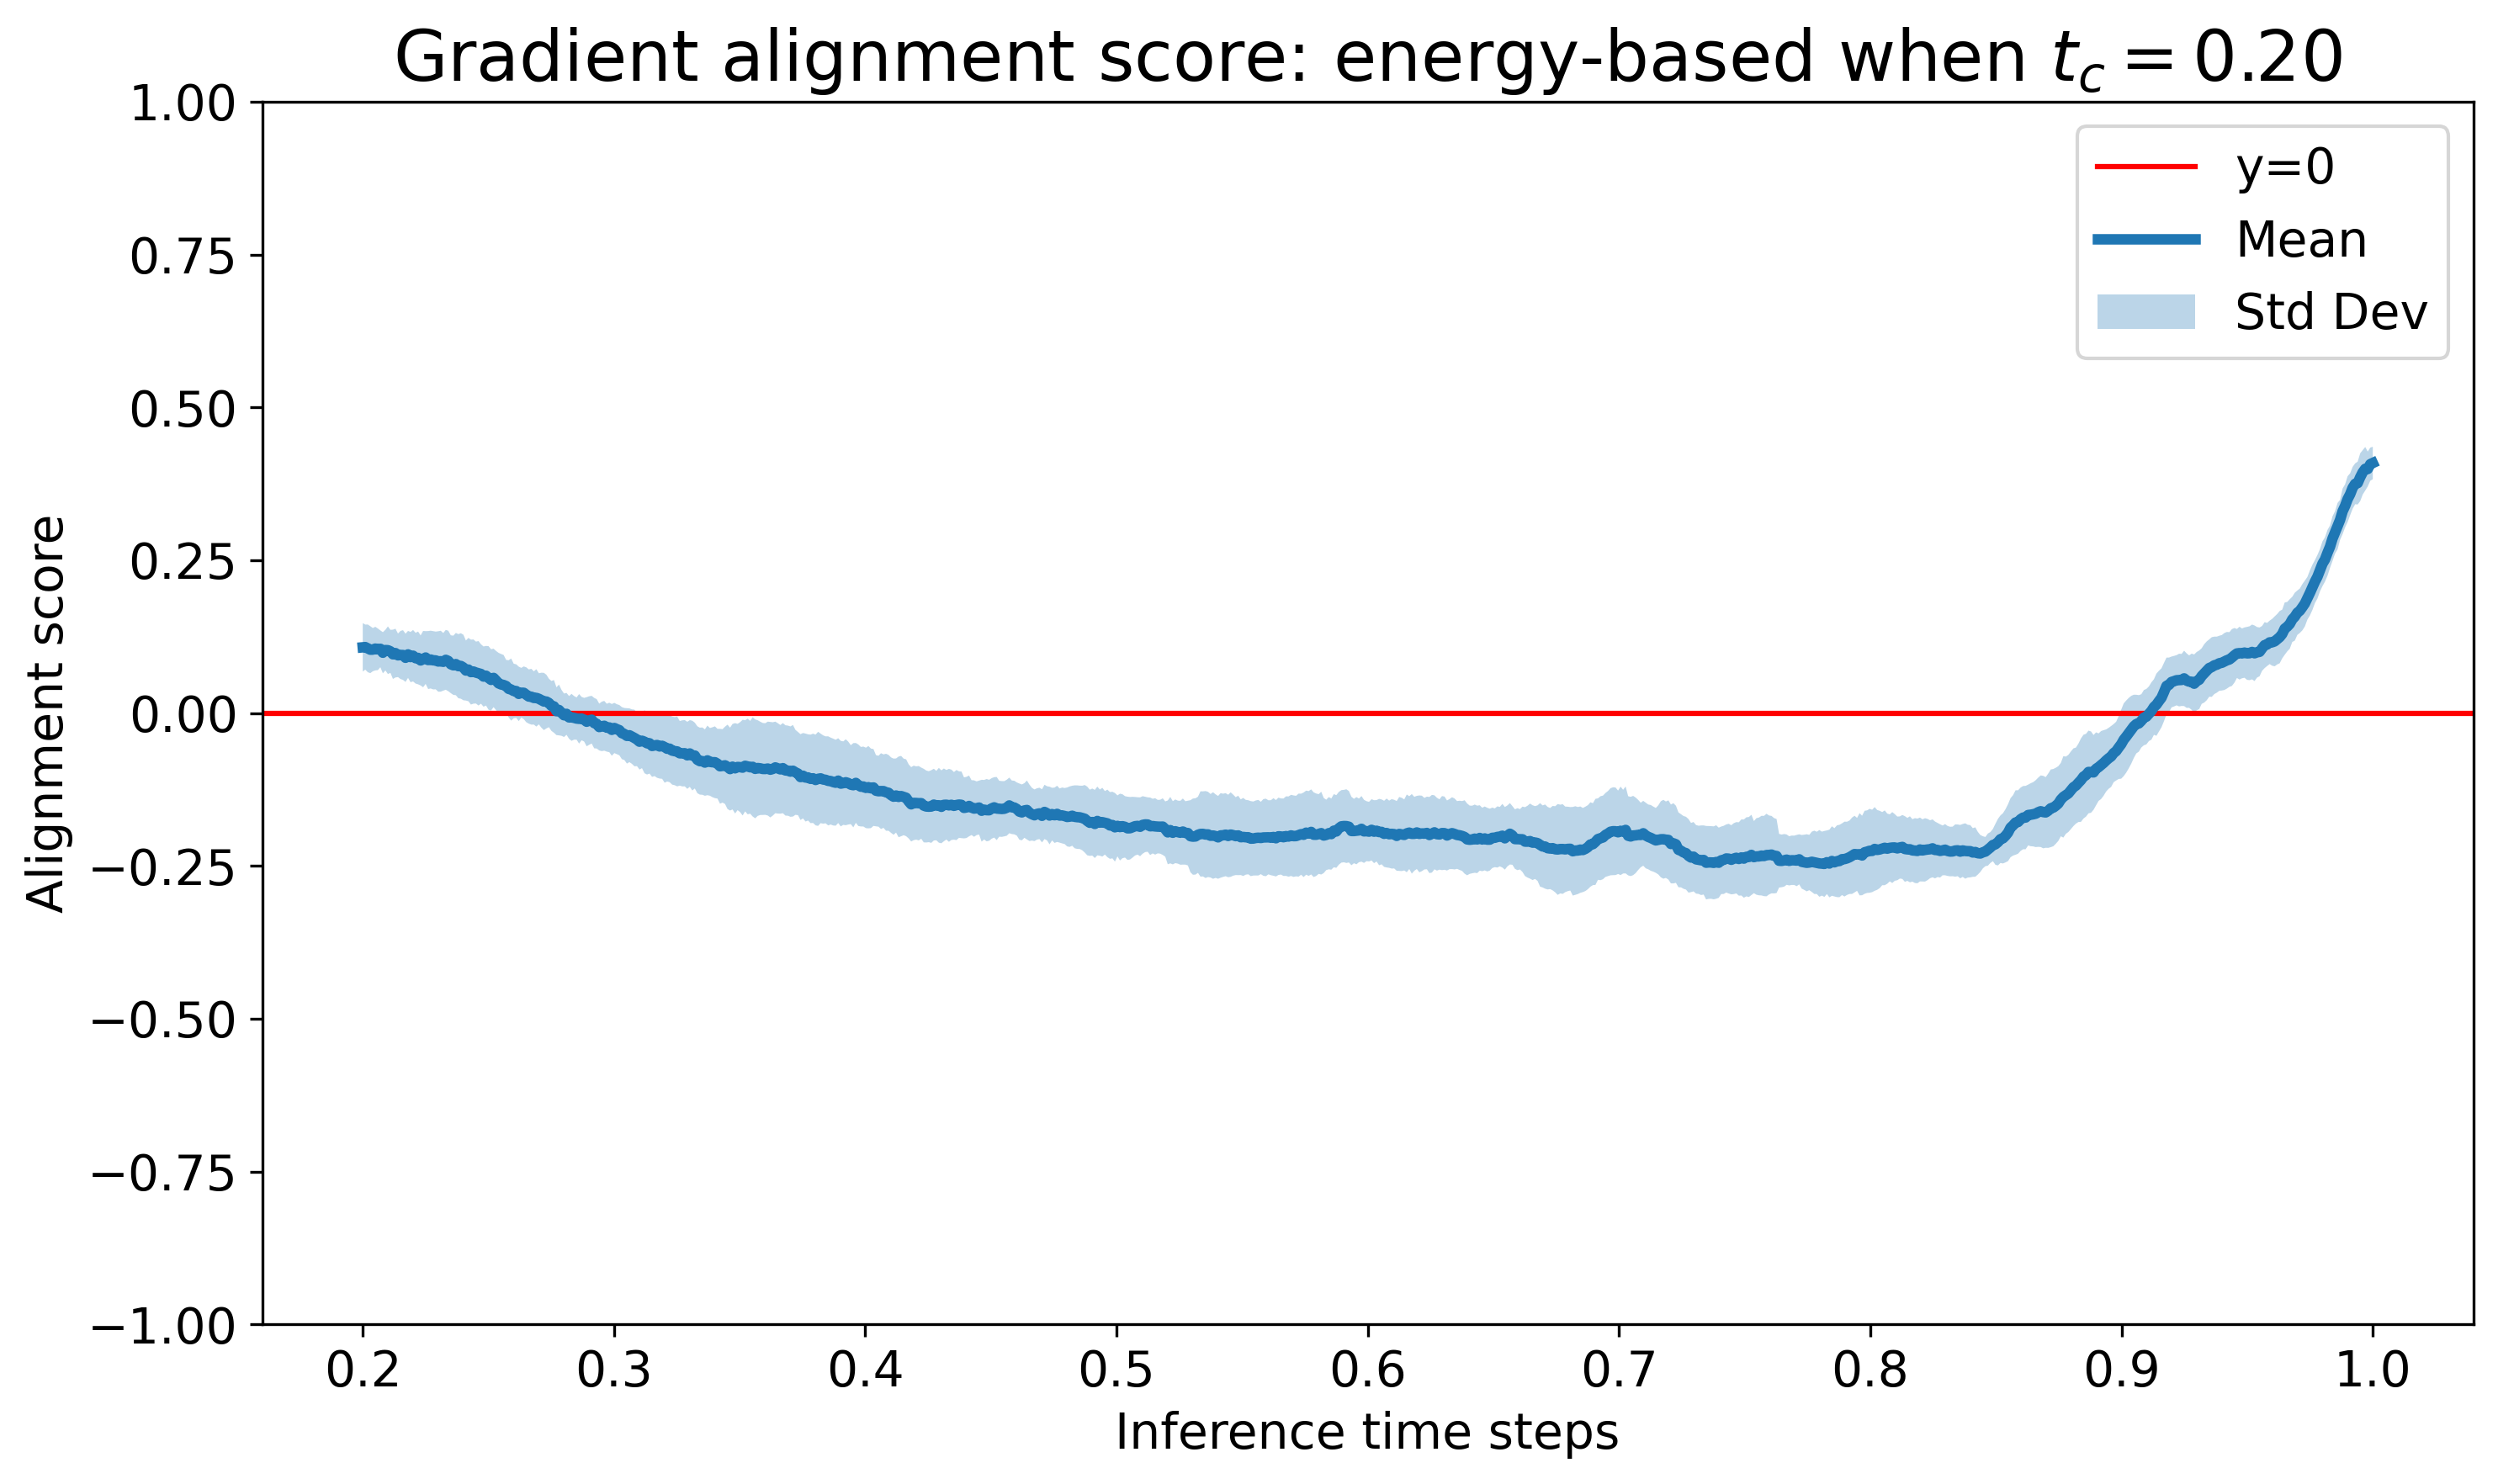
\includegraphics[width=0.45\textwidth]{chapter7/fig/mean_std_alignment_history_0.2.png}%
    }
    \subfloat[Physics injection when $t_c=0.6$]{%
        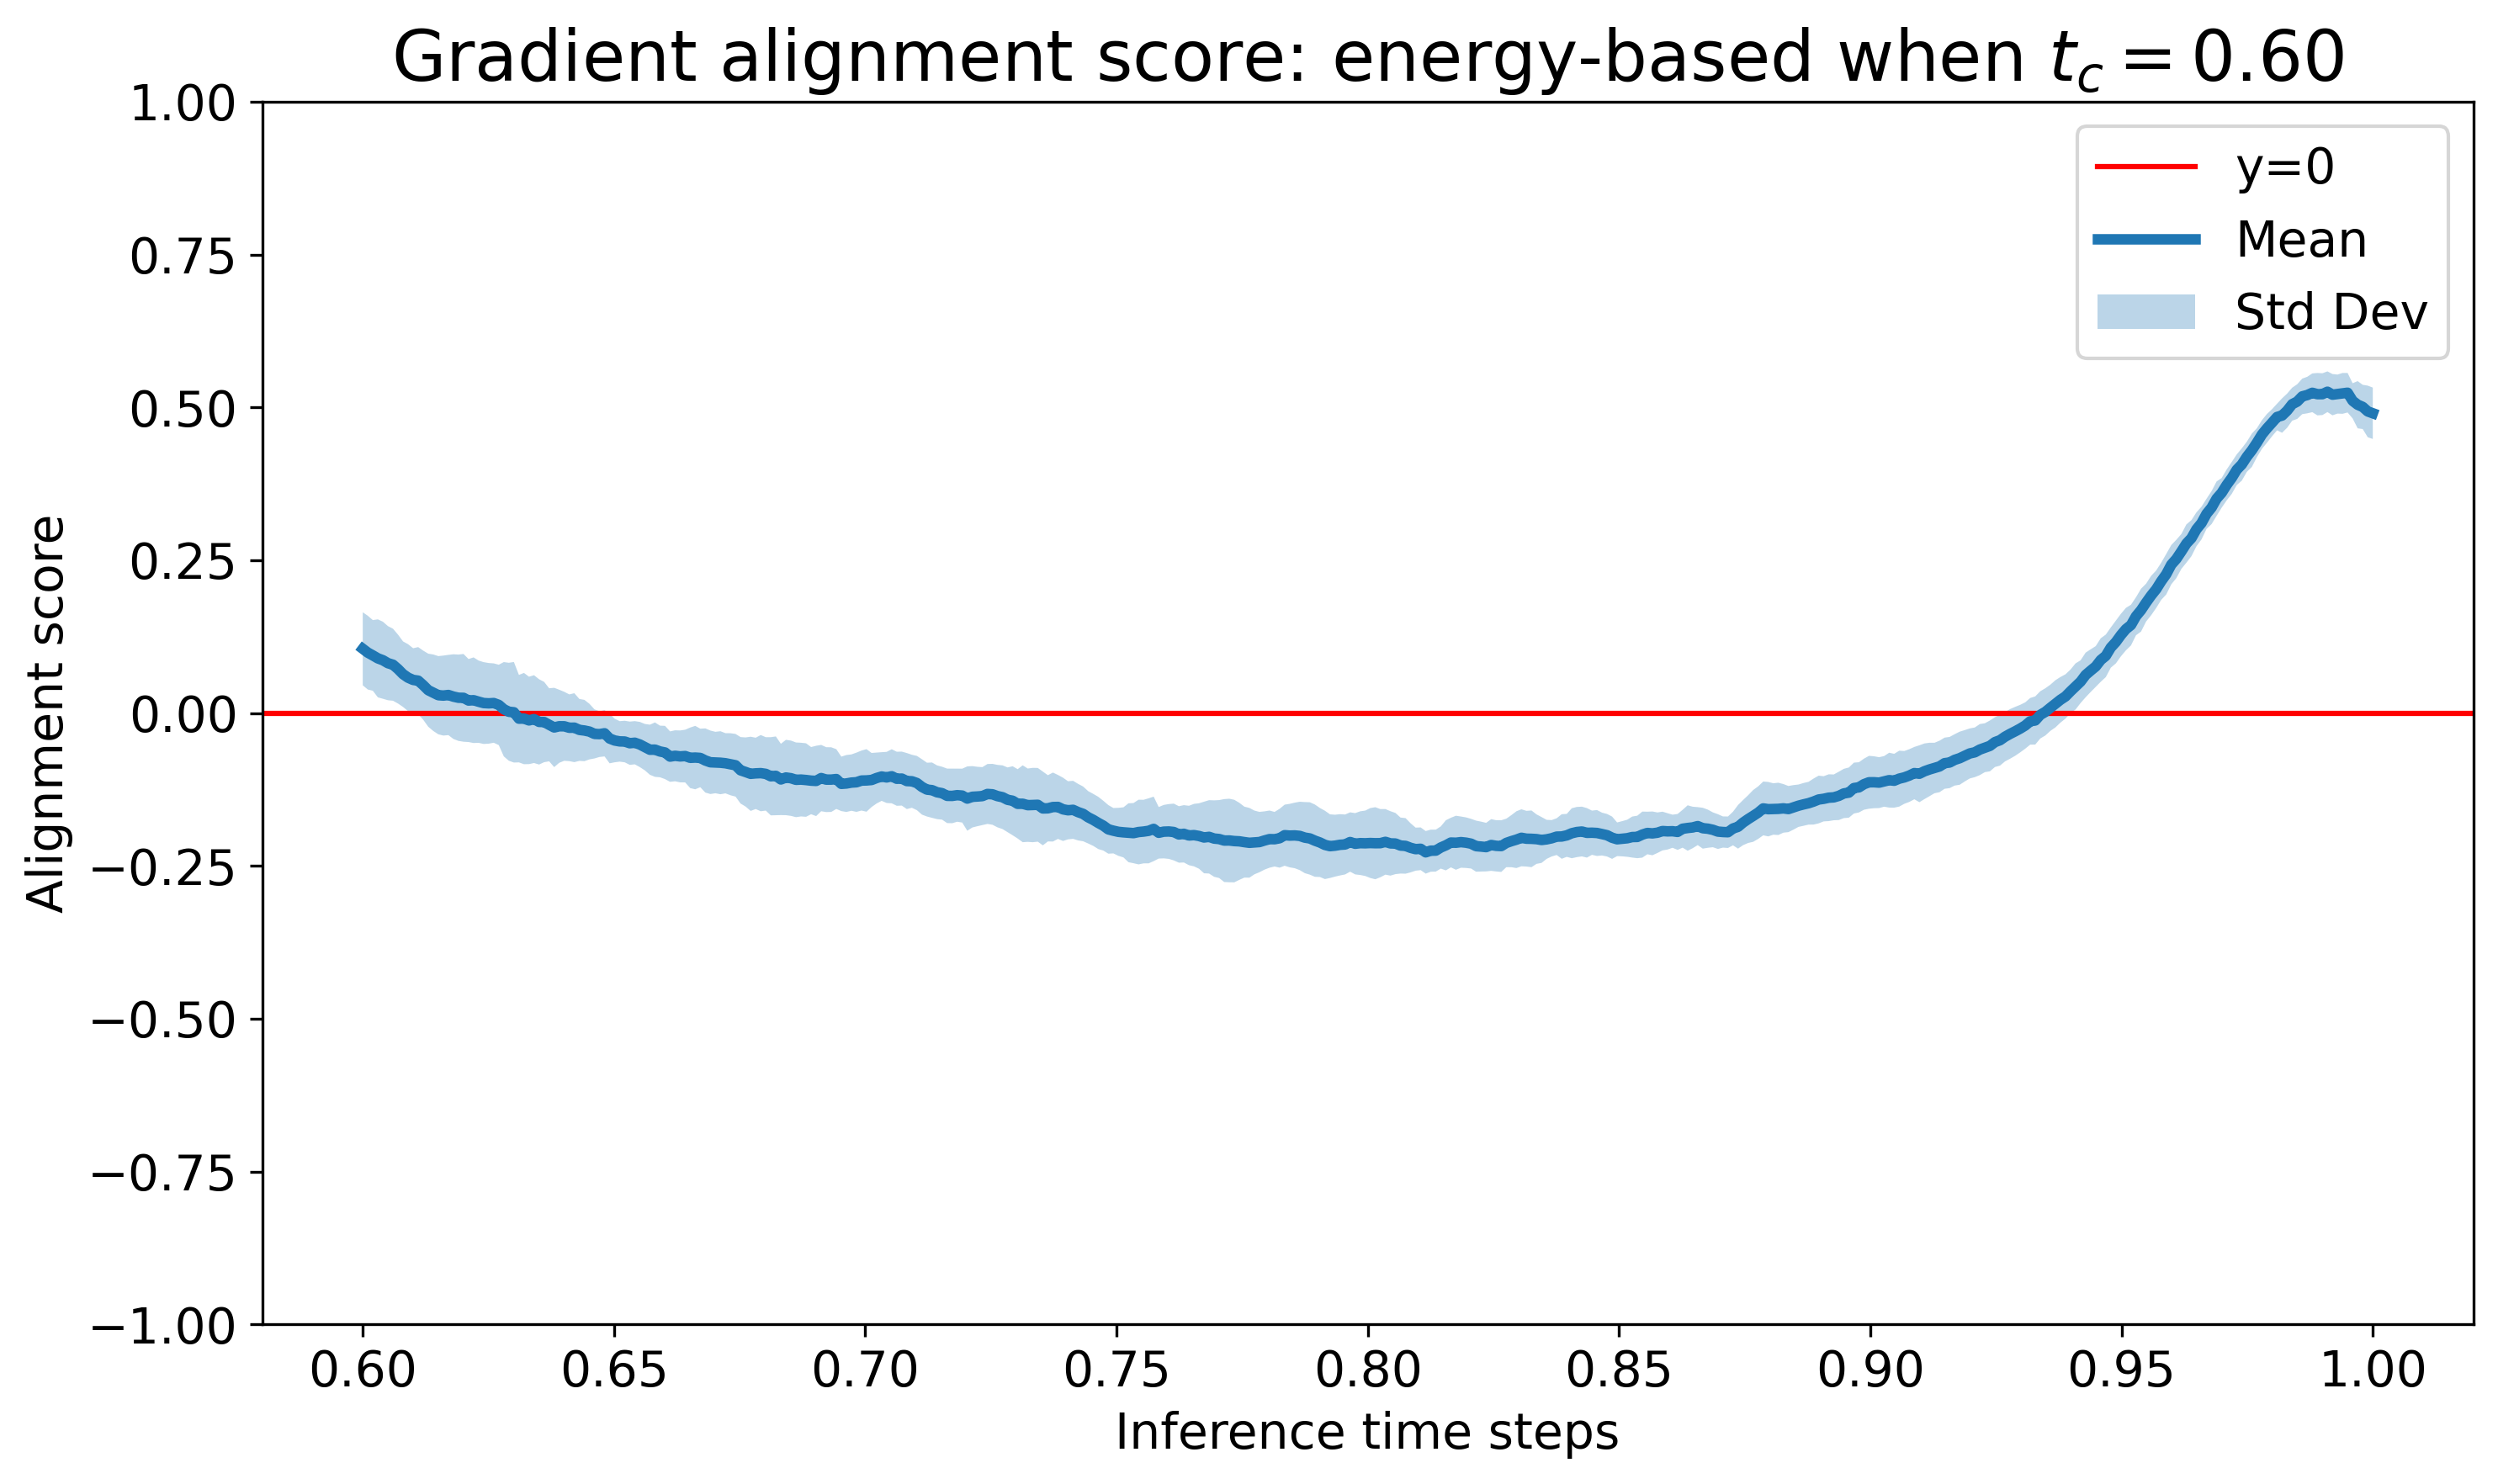
\includegraphics[width=0.45\textwidth]{chapter7/fig/mean_std_alignment_history_0.6.png}%
    }\\
    \subfloat[Physics injection when $t_c=0.8$]{%
        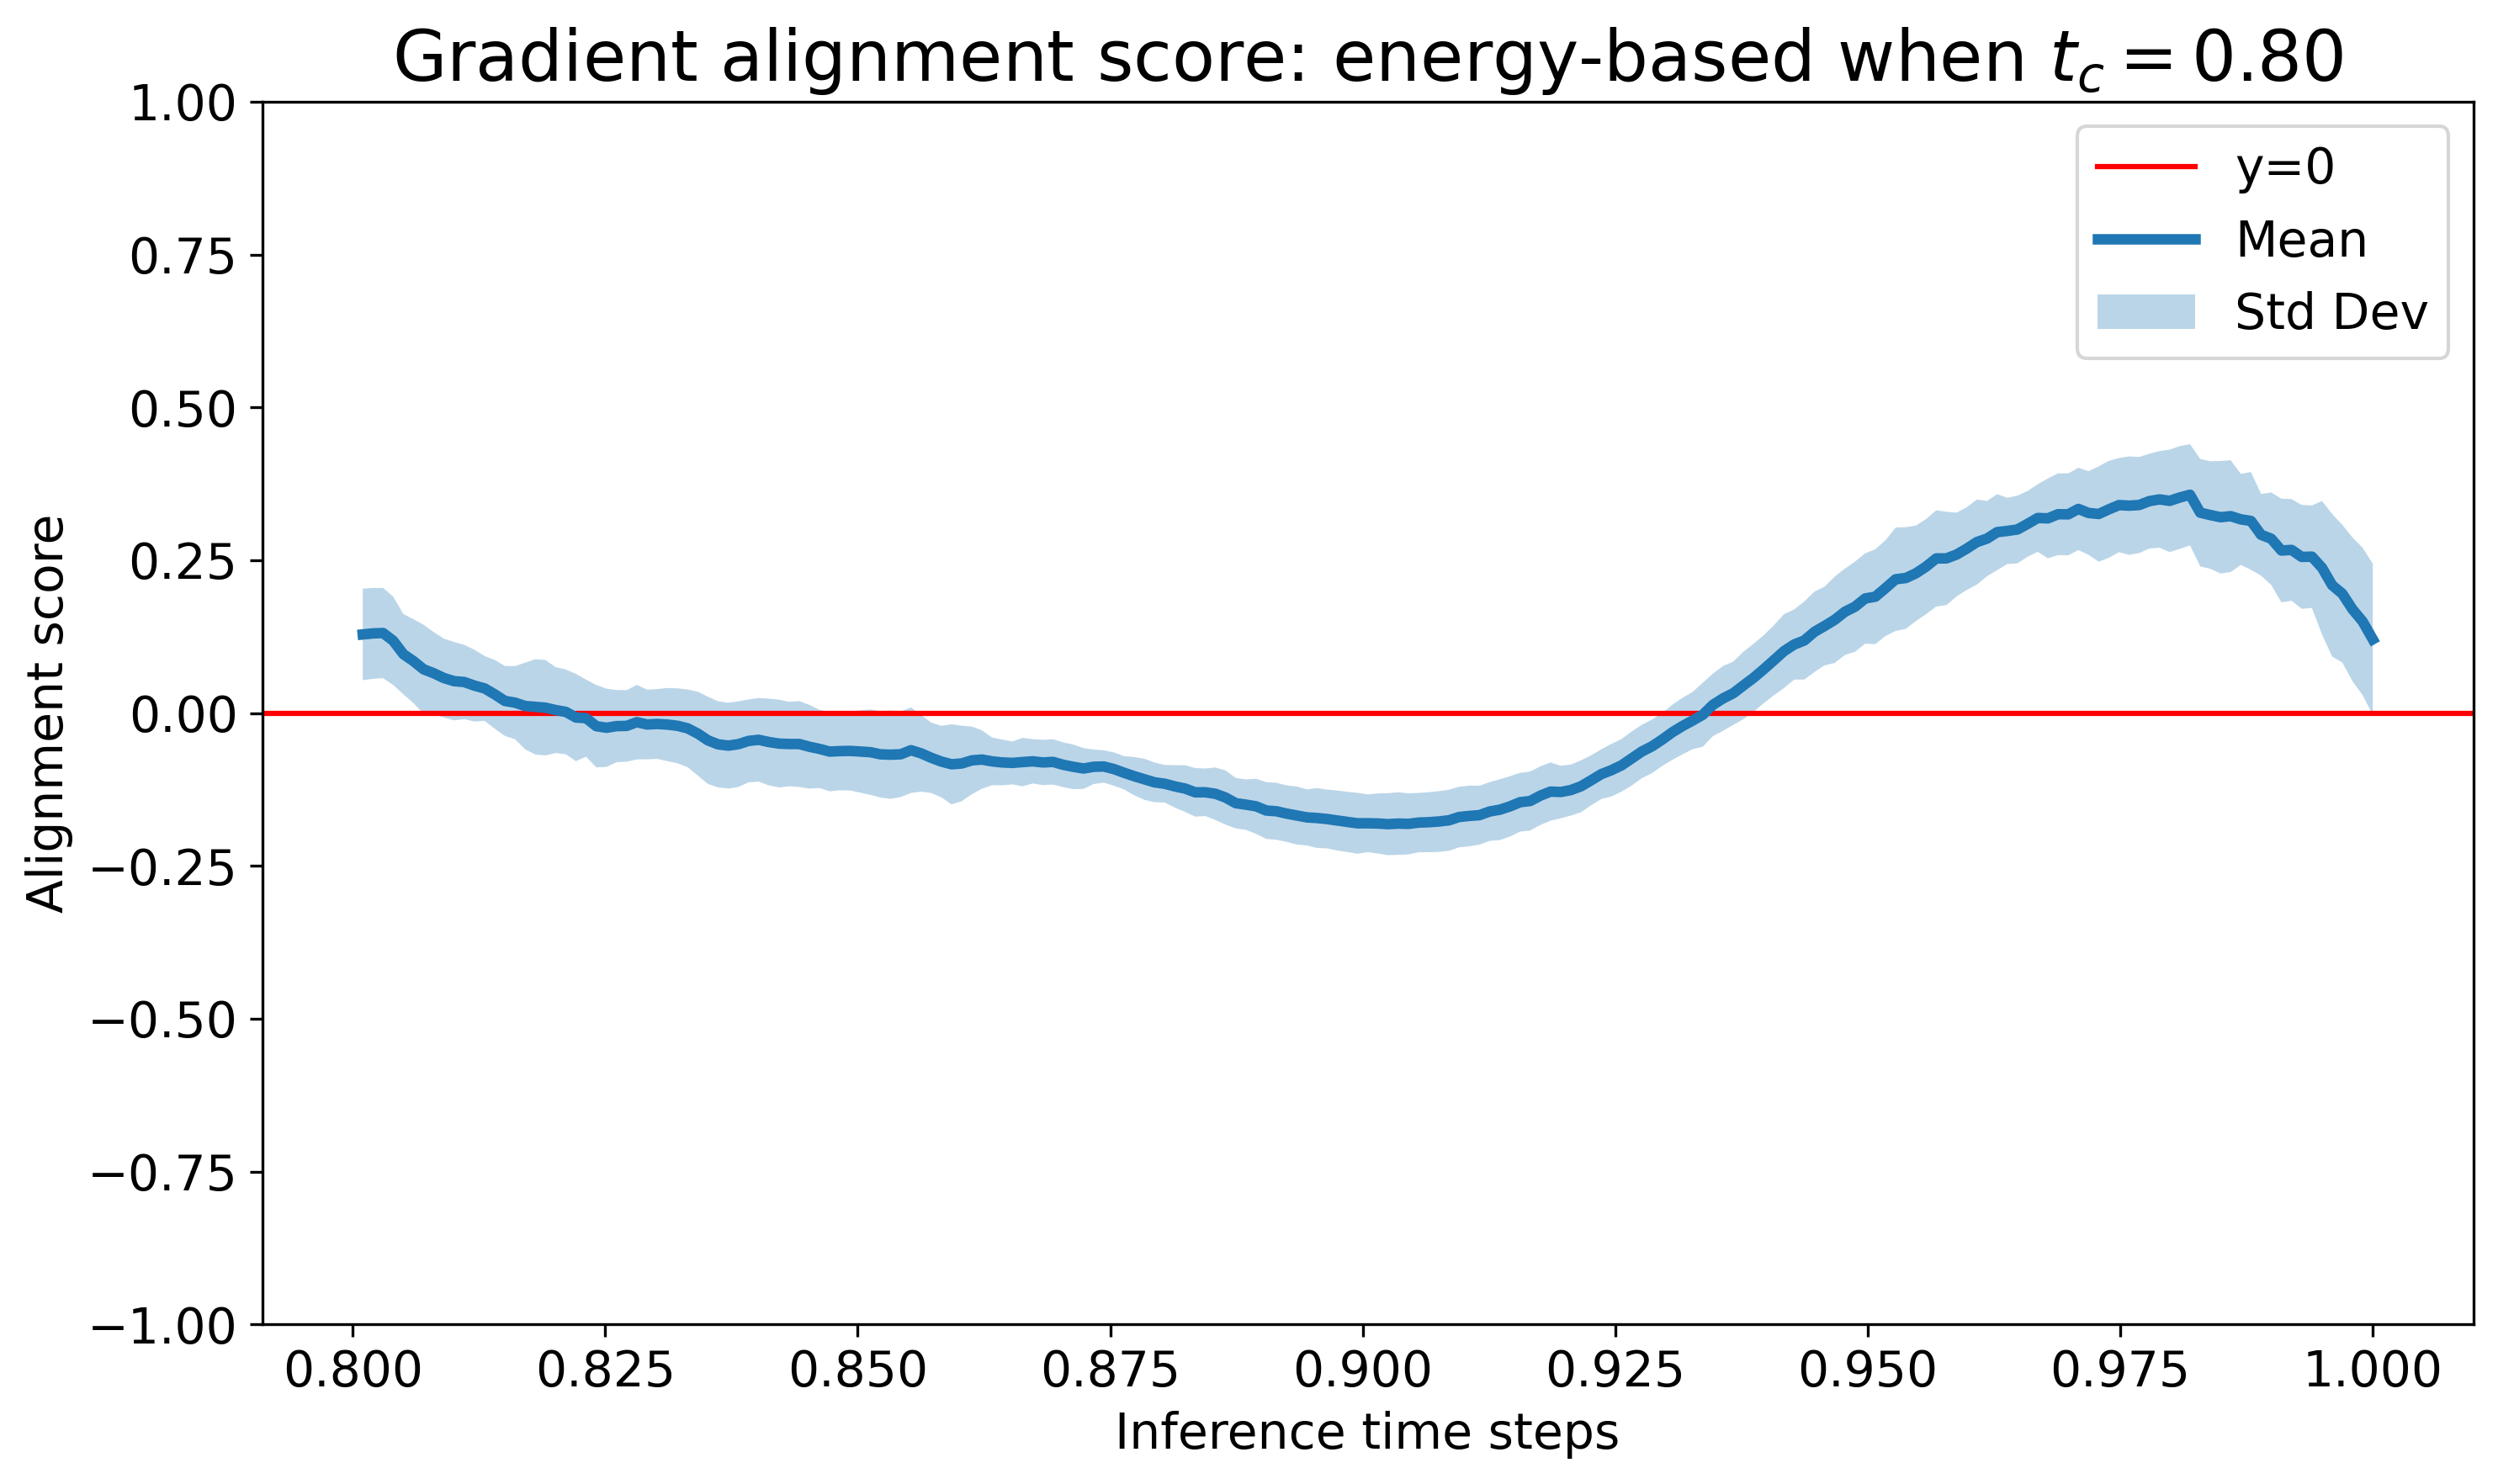
\includegraphics[width=0.45\textwidth]{chapter7/fig/mean_std_alignment_history_0.8.png}%
    }\quad
    \caption{Gradient alignment scores during the $\mathcal{L}_{\mathrm{phys}}$ injection phase of the energy-based inference ($T = 1000$, $\lambda = 10$) with varying $t_c$. 0 on $x$-axis indicates the onset of $\mathcal{L}_{\mathrm{phys}}$ injection.}
    \label{ch7:fig:alignmentScore_app}
\end{figure}


\begin{table}[!htb]
  \centering
  \renewcommand{\arraystretch}{1}
  \caption{Model performance comparison across methods and inference time steps ($T$).}
  \begin{tabular}{lcccc}
    \toprule
    \textbf{Method} & \textbf{T} & \textbf{$\mathcal{L}_{\mathrm{phys}}$} & \textbf{$C_L$} & \textbf{Time cost (s)} \\
    \midrule
    \multirow{1}{*}{Conditional training}
      & 2000  & $(5.35 \pm 0.86)\times10^{-3}$ & $0.627 \pm 0.028$ & 12779.44 \\
    \midrule
    \multirow{3}{*}{Energy-based ($t_c=0.0$)}
      & 200   & 0.1766         & 0.1957           & 6678.79 \\
      & 1000  & $(1.07 \pm 0.60)\times10^{-2}$ & $0.655 \pm 0.023$ & 3169.04 \\
      & 2000  & $(4.69 \pm 0.86)\times10^{-2}$ & $0.553 \pm 0.026$ & 6779.44 \\
    \midrule
    \multirow{3}{*}{Energy-based ($t_c=0.2$)}
      & 200   & 0.0927         & 0.1373           & 5395.10 \\
      & 1000  & $(1.51 \pm 0.79)\times10^{-3}$ & $0.683 \pm 0.008$ & 3192.07 \\
      & 2000  & $(1.22 \pm 0.10)\times10^{-2}$ & $0.596 \pm 0.005$ & 6002.10 \\
    \midrule
    \multirow{3}{*}{Energy-based ($t_c=0.6$)}
      & 200   & 0.0716         & 0.1407           & 3342.80 \\
      & 1000  & $(4.80 \pm 6.91)\times10^{-4}$ & $0.710 \pm 0.0045$ & 3136.75 \\
      & 2000  & $(4.24 \pm 0.81)\times10^{-3}$ & $0.639 \pm 0.006$ & 6485.92 \\
    \midrule
    \multirow{3}{*}{Energy-based ($t_c=0.8$)}
      & 200   & 0.0361         & 0.1748           & 1186.29 \\
      & 1000  & $(8.40 \pm 4.0)\times10^{-4}$  & $0.721 \pm 0.004$ & 3015.18 \\
      & 2000  & $(9.54 \pm 1.20)\times10^{-3}$ & $0.703 \pm 0.017$ & 6440.14 \\
    \midrule
    \textbf{Dflow-SUR} & \textbf{50} & \boldmath{$(4.80 \pm 6.91)\times10^{-8}$} & \boldmath{$0.699 \pm 6\times10^{-9}$} & \textbf{801} \\
    \bottomrule
  \end{tabular}
  \label{ch7:tab:modelPerformanceResults}
\end{table}

\begin{figure}[!htbp]
    \centering
    \subfloat[Physics injection when $t_c=0.0$]{%
        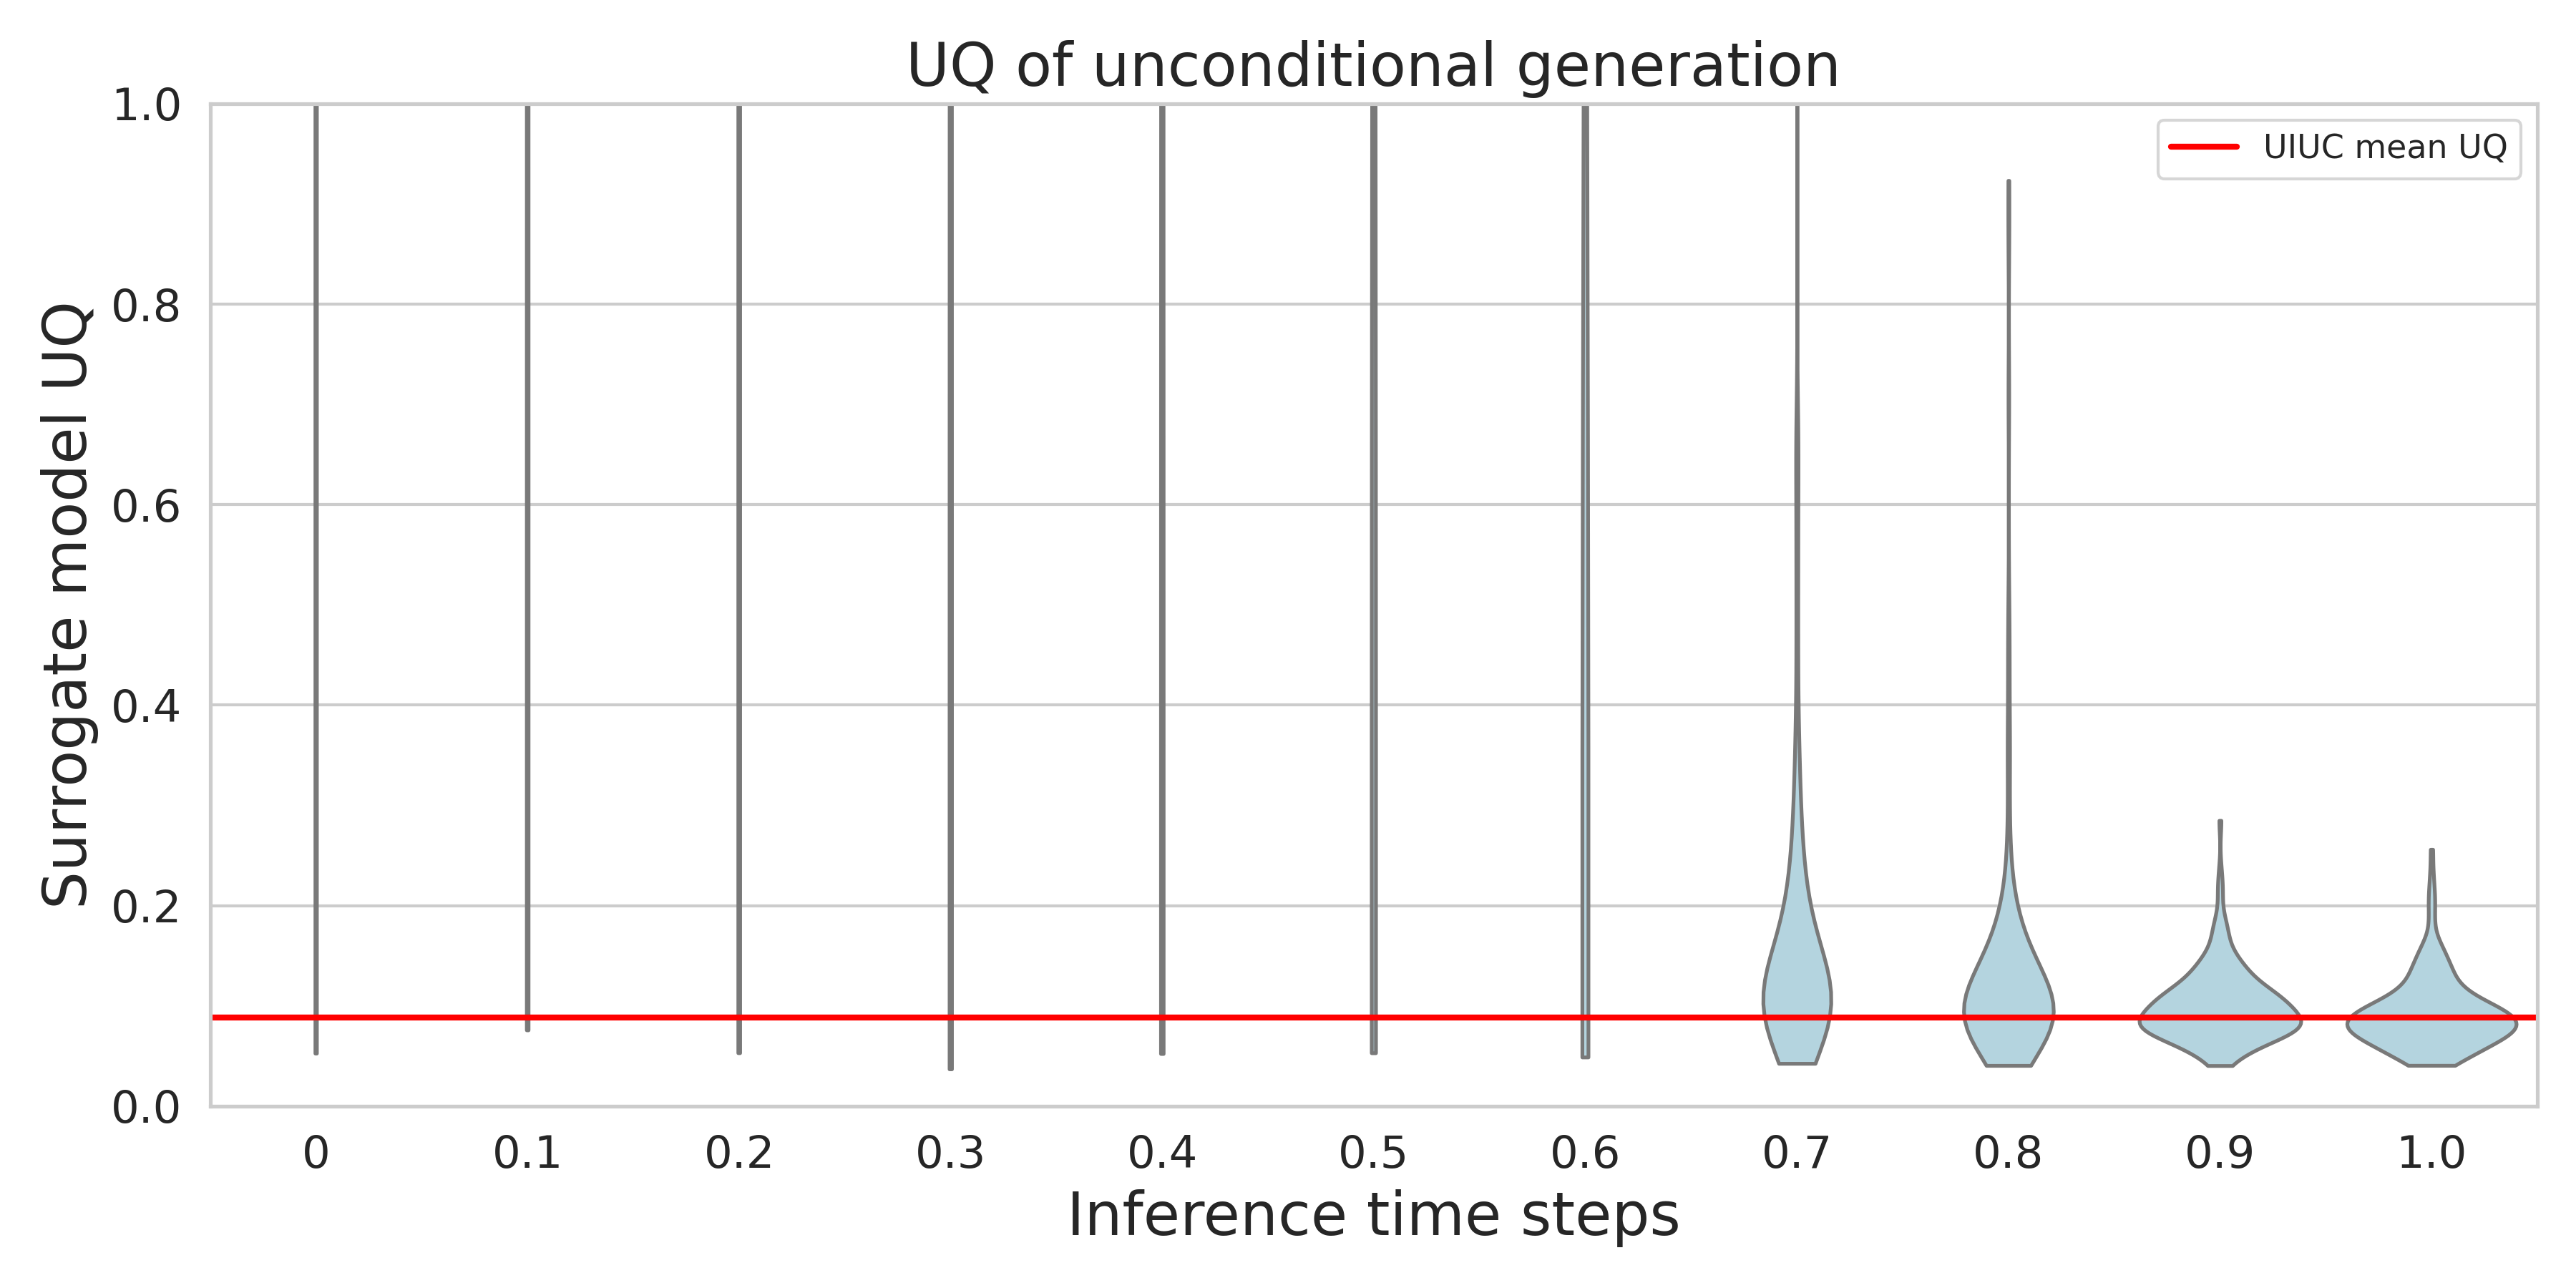
\includegraphics[width=0.5\textwidth]{chapter7/fig/energy_T_0.0_violin_std.png}%
    }
    \subfloat[Physics injection when $t_c=0.2$]{%
        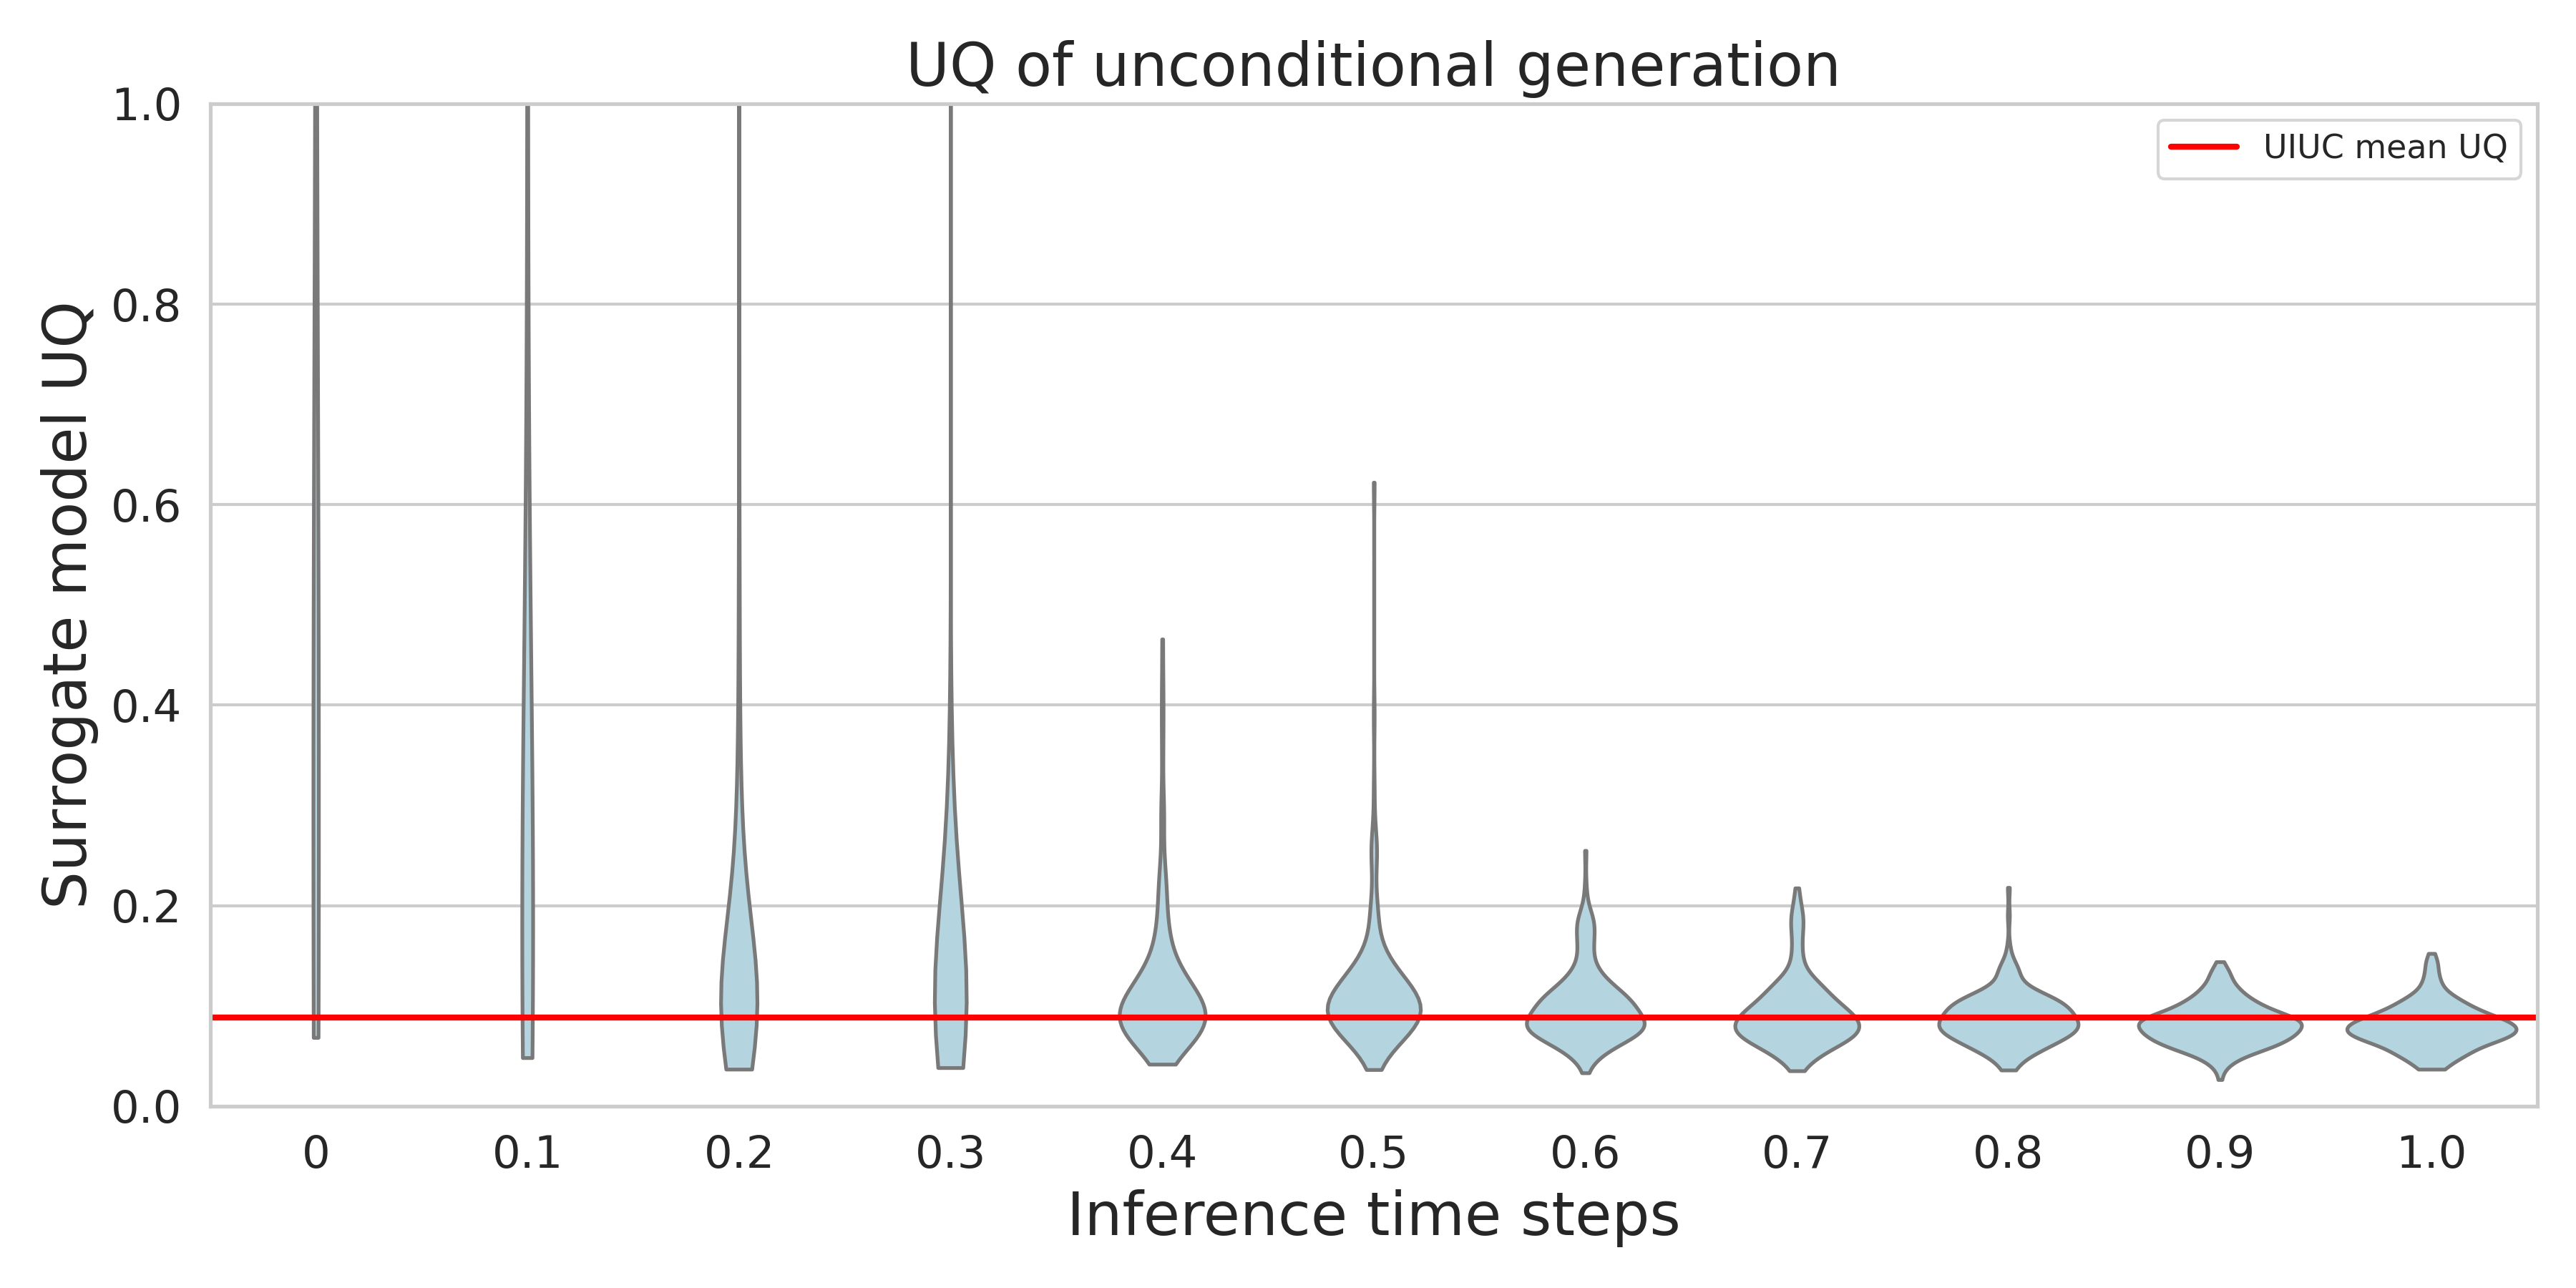
\includegraphics[width=0.5\textwidth]{chapter7/fig/energy_T_0.2_violin_std.png}%
    }\\[1em]
    \subfloat[Physics injection when $t_c=0.6$]{%
        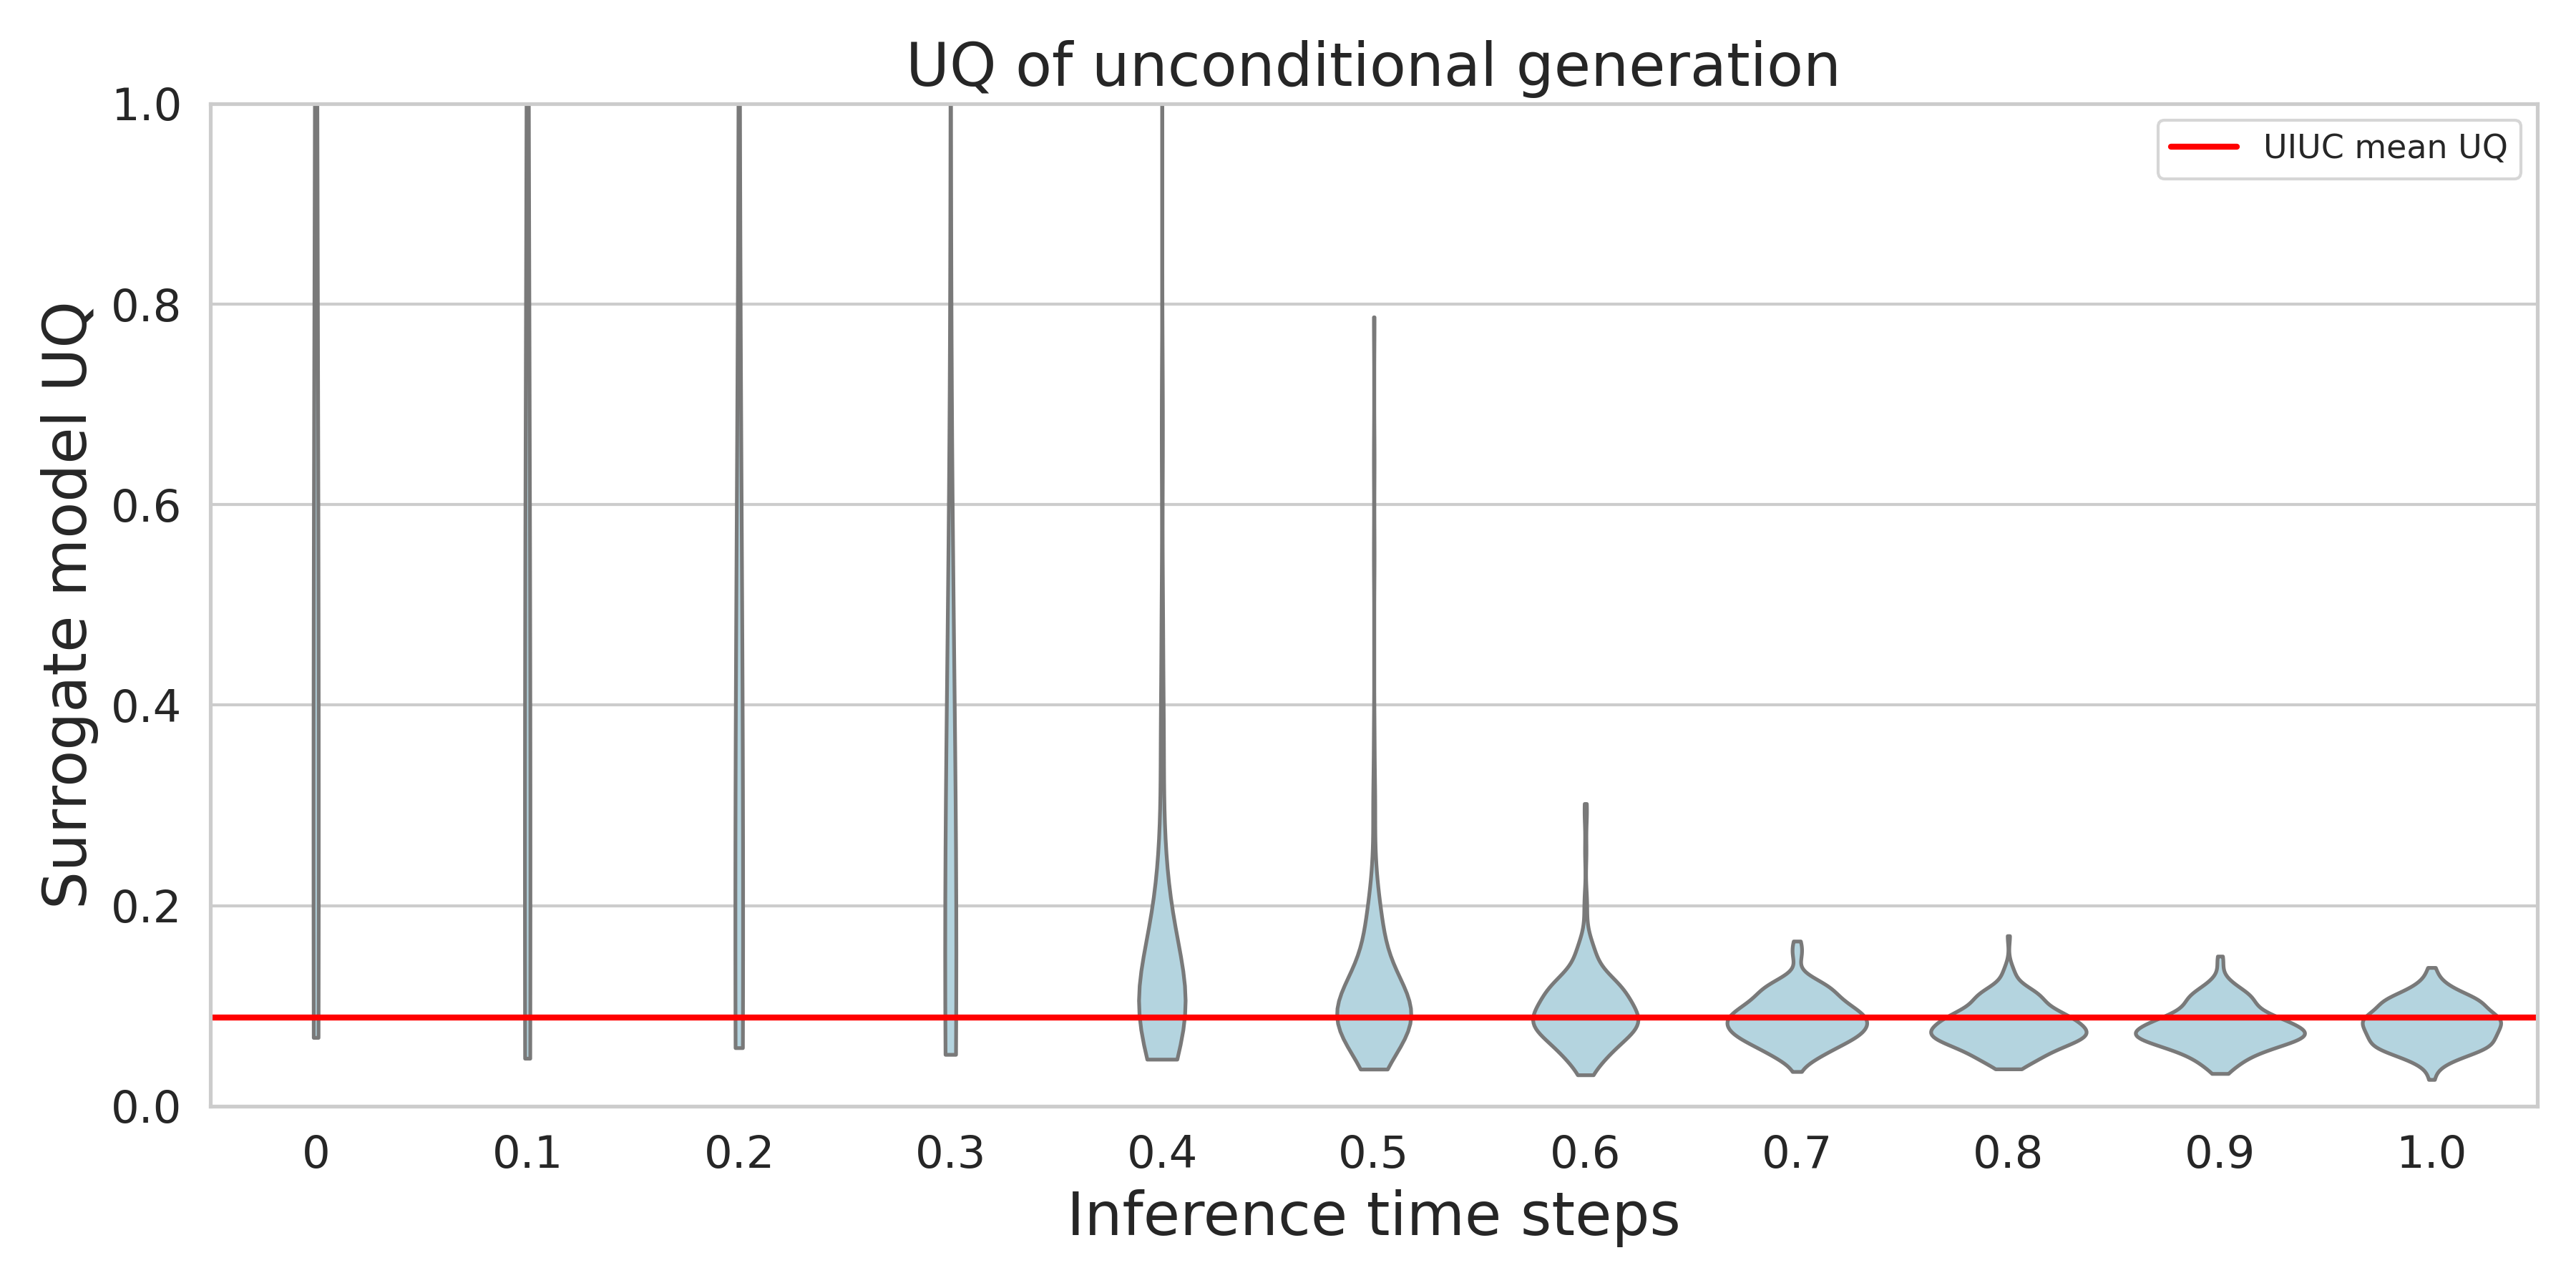
\includegraphics[width=0.5\textwidth]{chapter7/fig/energy_T_0.6_violin_std.png}%
    }
    \subfloat[Physics injection when $t_c=0.8$]{%
        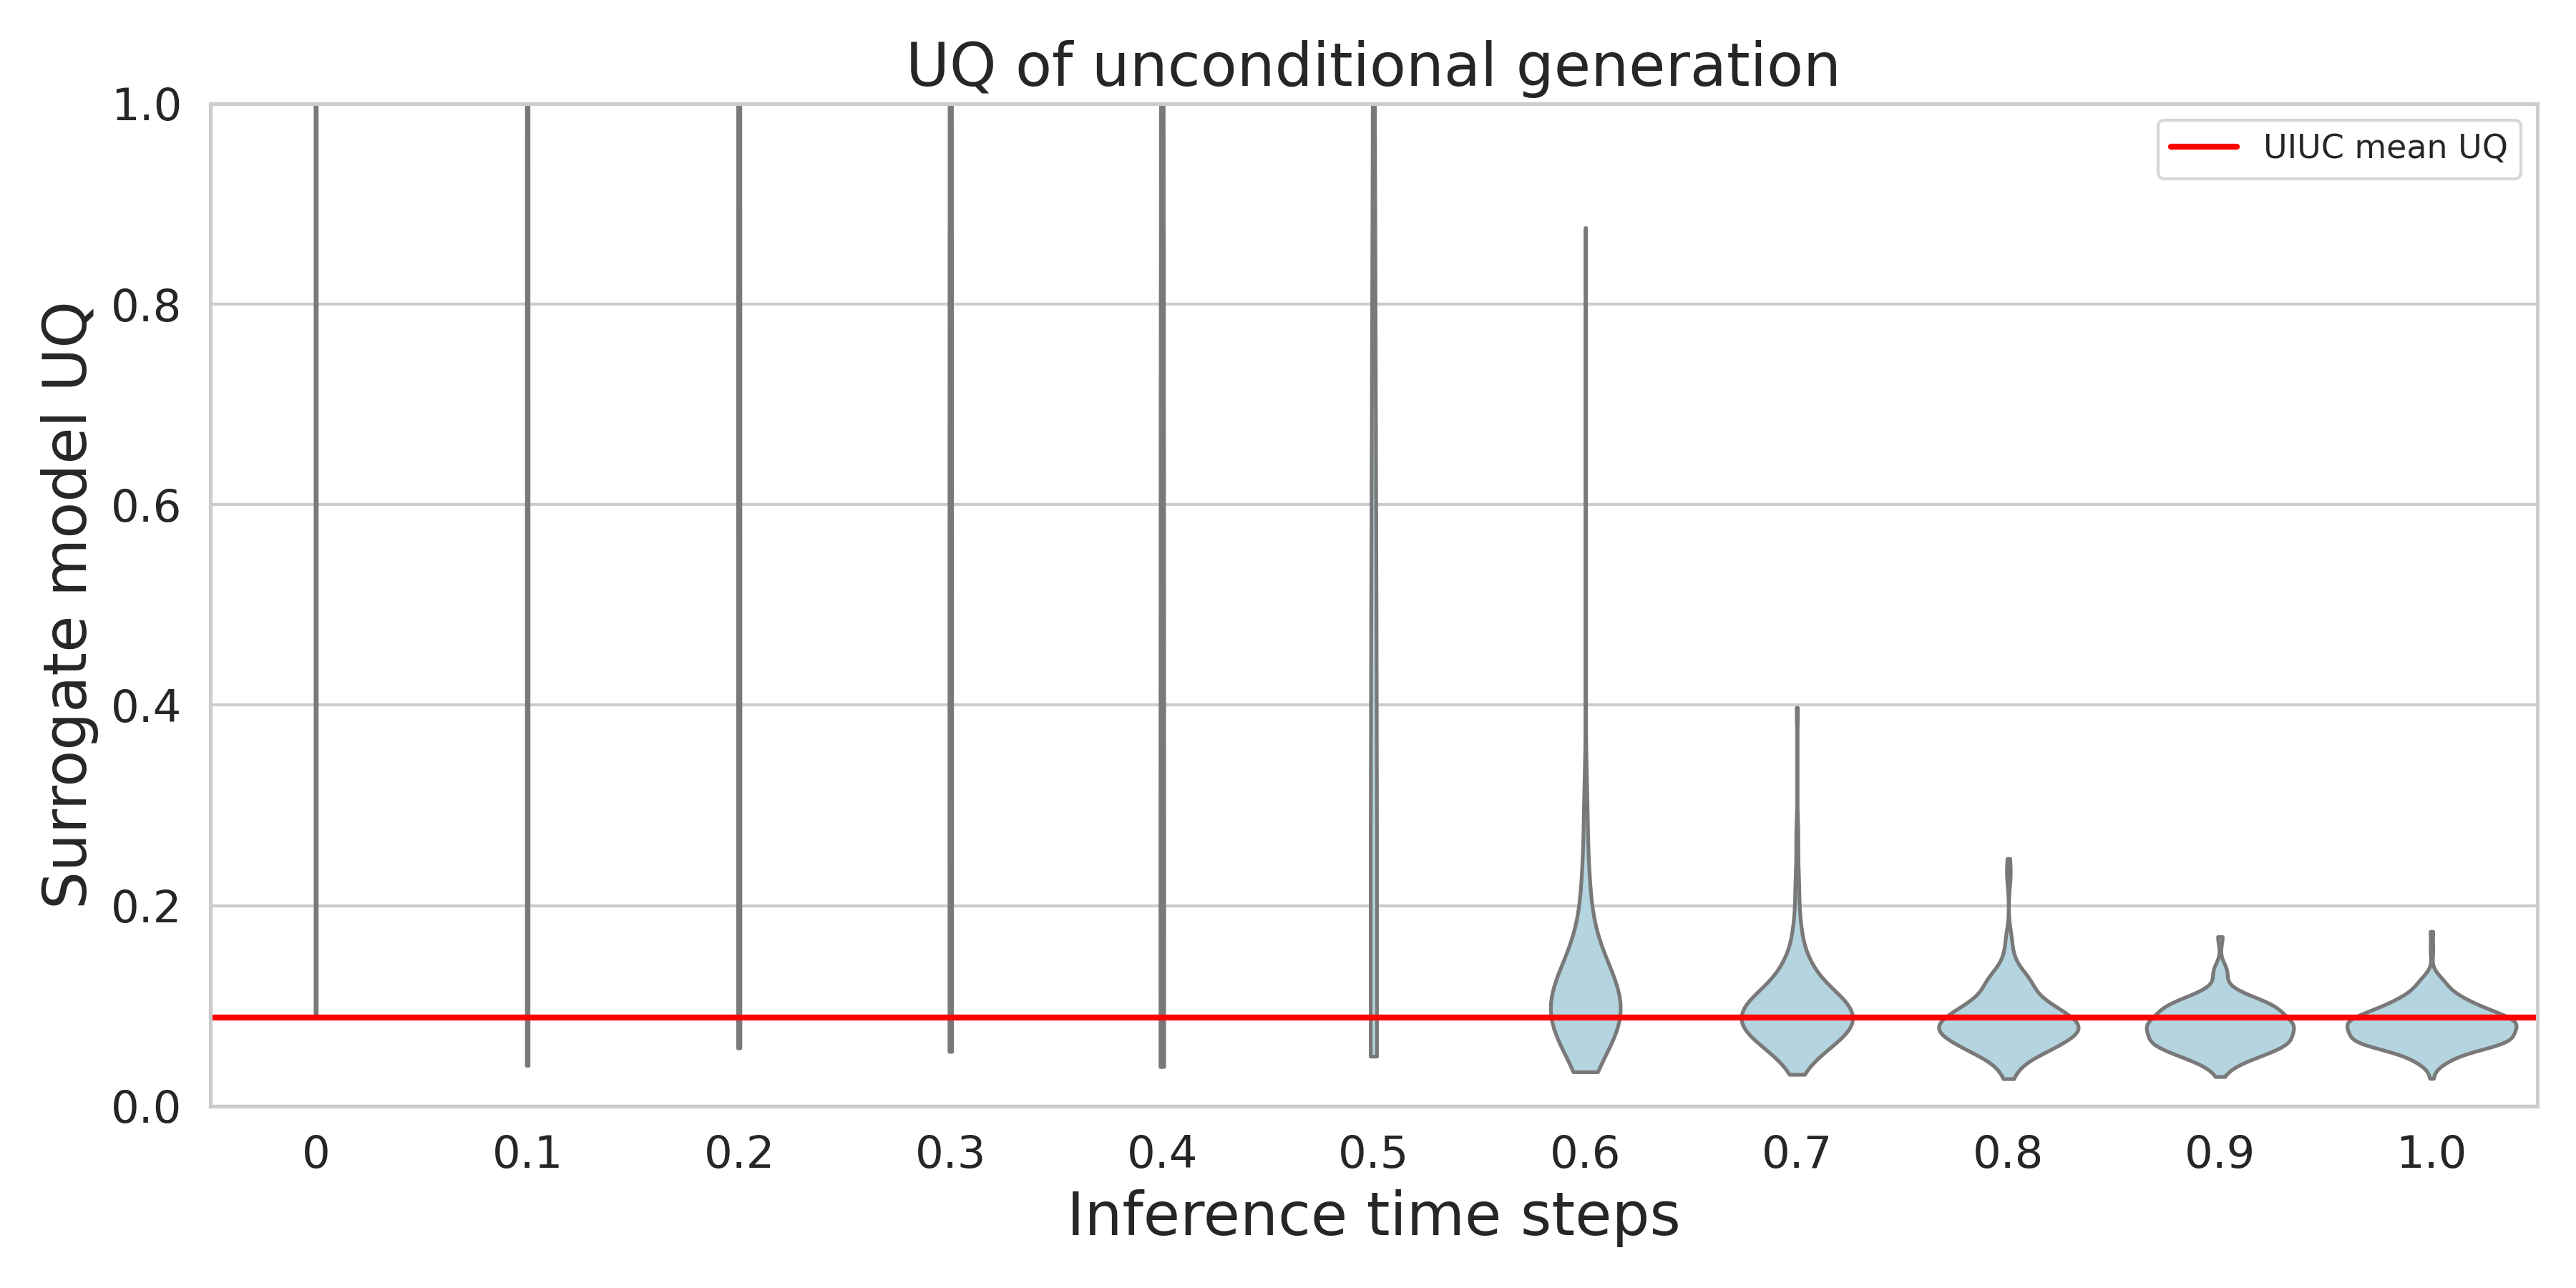
\includegraphics[width=0.5\textwidth]{chapter7/fig/energy_T_0.8_violin_std.png}%
    }
    \caption{UQ of generative samples for energy-based approach (total inference time step = 1000) with various $T$ physics injection (the red line represents the UIUC data UQ mean).}
    \label{ch7:fig:uqEnergy}
\end{figure}


\subsubsection{UQ of energy-based approach}
\label{ch7:sect:AppendixUncertainty}

We further present the UQ of generated samples from the energy-based approach evaluated by the surrogate model at each inference time step in Figure~\ref{ch7:fig:uqEnergy}. From analyzing the figures, we can observe that samples generated by the energy-based method during its generation process still exhibit high surrogate-evaluated UQ in the inference phase, thereby misleading the loss guidance.